\clearpage

\lehead[]{\normalfont\sffamily\hspace*{-2.00cm}\textcolor{white}{\colorbox{lightblue}{\parbox[c][0.70cm][b]{1.60cm}{
\makebox[1.60cm][r]{\thechapter}\\ \makebox[1.60cm][r]{ÜBUNG}}}}\hspace{0.17cm}\textcolor{lightblue}{\chaptertitle}}
\rohead[]{\textcolor{lightblue}{\chaptertitle}\normalfont\sffamily\hspace*{0.17cm}\textcolor{white}{\colorbox{lightblue}{\parbox[c][0.70cm][b]{1.60cm}{\thechapter\\
ÜBUNG}}}\hspace{-2.00cm}}
%\chead[]{}
\rehead[]{\textcolor{lightblue}{AvHG, Inf, My}}
\lohead[]{\textcolor{lightblue}{AvHG, Inf, My}}

\section{Arrays -- Übungen}

\subsection{Aufgabe 1: Zahlen}

\begin{compactenum}[a)]
\item Erstelle ein neues Java-Anwendungsfenster. Lege eine globale Variable
für ein Array von \lstinline|int|-Werten an und erzeuge ein Feld mit 100
Elementen. Fülle das Zahlenarray im Konstruktor mit Zahlen von 100 bis 199.

\item  Gib in einer Zeile im Anwendungsfenster die ersten 10 Zahlen des
Arrays aus:


\includegraphics[width=0.6\textwidth]{./inf/SEKII/18_Java_Arrays/Aufgabe1a.png}

\item Erweitere die Ausgabe so, dass alle Zahlen des Arrays zeilenweise
untereinander ausgegeben werden. Jeweils 10 Zahlen sollen in einer Zeile stehen.

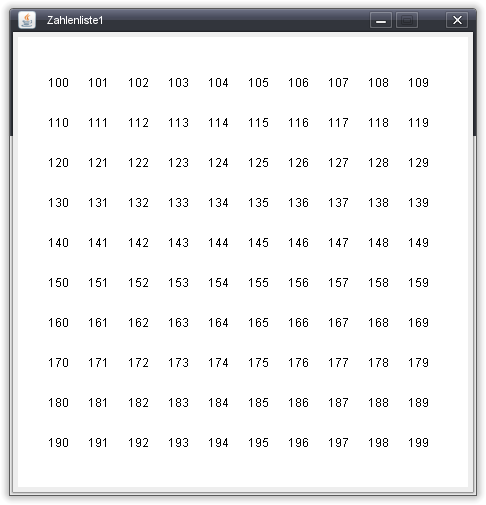
\includegraphics[width=0.8\textwidth]{./inf/SEKII/18_Java_Arrays/Aufgabe1b.png}

\item Wenn du willst kannst du nun Versuchen diese Aufgabe mit einem
zweidimensionalen Array statt mit einem eindimensionalen Array zu lösen.
\end{compactenum}

\subsection{Aufgabe 2: Summe und Extremwerte von Zahlen}

\begin{compactenum}[a)]
\item Erstelle ein neues Java-Anwendungsfenster. Erzeuge ein
\lstinline|int|-Array mit 10 Elementen und schreibe im Konstruktor das
Anwendungsfensters in das Array Zahlen von 1 bis 10. Gib die 10 Zahlen in einer
Zeile des Anwendungsfensters aus.

\item Verändere das Programm so, dass in jedes Feld das Arrays im Konstruktor
mit einer Zufallszahl zwischen 1 und 100 gefüllt wird.

\begin{minipage}{0.35\textwidth}
\item Berechne die Summe aller Zahlen und gib sie im Anwendungsfenster aus.

\item Ermittle die kleinste Zahl des Arrays und gib sie im Anwendungsfenster
aus.

\item Ermittle die größte Zahl des Arrays und gib sie im Anwendungsfenster aus.
\end{minipage}
\hfill
\begin{minipage}{0.65\textwidth}
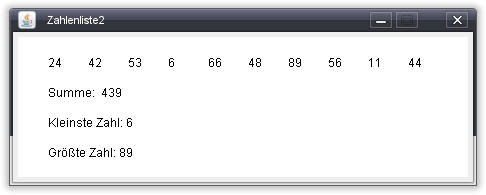
\includegraphics[width=1.0\textwidth]{./inf/SEKII/18_Java_Arrays/Aufgabe2.png}
\end{minipage}
\end{compactenum}


\subsection{Aufgabe 3: Strichmännchen}

Vor einiger Zeit hast du eine Klasse \myClass{Strichmaennchen} programmiert und
eigene Strichmännchen über den Bildschirm laufen lassen. Erweitere das alte
Anwendungsprogramm so, dass du ein Array von 20 Strichmännchen erzeugst.
Generiere dabei für die y-Position und für die Geschwindigkeit des
Strichmännchens Zufallswerte, damit die Strichmännchen an unterschiedlichen
Positionen erscheinen und unterschiedlich schnell laufen.


\subsection{Aufgabe 4: Billardkugeln}

Benutze die Billardkugeln aus dem Kapitel über Vererbung. Erzeuge ein Array
von 50 oder mehr Billardkugeln, die über den Bildschirm rollen. Generiere für
die x-Position, die y-Position und die Geschwindigkeitswerte der Billardkugeln
geeignete Zufallswerte.


\subsection{Aufgabe 5: Meer mit Fischen}

Ein Schwarm von Fischen schwimmt wild durcheinander. Dazu findest du im
Kursrepository verschiedene animierte Bilder von Fischen.

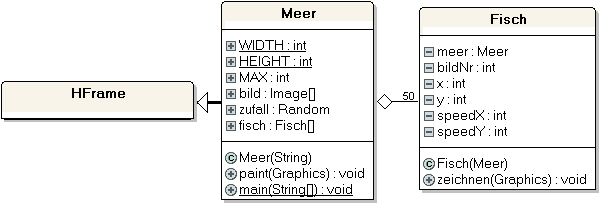
\includegraphics[width=1.0\textwidth]{./inf/SEKII/18_Java_Arrays/Aufgabe5a.png}

\begin{compactenum}[a)]
\item Erzeuge ein großes Anwendungsfenster mit der Hintergrundfarbe cyan.
Generiere im Anwendungsfenster einen Zufallsgenerator (ein Objekt der Klasse
\myClass{Random}) und lade alle Fisch-Bilder, die du verwenden möchtest, in ein
Array vom Typ \myClass{Image}. Außerdem soll ein Array von 50 Objekten der
Klasse \myClass{Fisch} erzeugt werden, die in Teil b) programmiert wird.

\emph{Anmerkung}: Auf ein Objekt der Klasse \myClass{Timer} kann man verzichten,
weil das Fenster durch die animierten Bilder automatisch regelmäßig neu
gezeichnet wird.

\item Programmiere eine Klasse \myClass{Fisch}. Der einzige Parameter, der im
Konstruktor übergeben wird, ist ein Objekt des Anwendungsfensters. Über dieses
Objekt kann man beim Zeichnen auf die Bilder zugreifen und man kann die Breite
und Höhe des Fensters abfragen (\lstinline|WIDTH|, \lstinline|HEIGHT|).

Im Konstruktor werden die Eigenschaften eines Fisches mit Zufallswerten
festgelegt. Verwende dazu den Zufallsgenerator aus dem Anwendungsfenster:

\begin{compactitem}
\item \lstinline|bildNr|: legt fest welches der Fisch-Bilder verwendet wird
\item \lstinline|x|: anfängliche x-Position (Wert zwischen 0 und
\lstinline|WIDTH|)
\item \lstinline|y|: anfängliche y-Position (Wert zwischen 20 und
\lstinline|HEIGHT|)
\item \lstinline|speedX|: Geschwindigkeit in x-Richtung. Wenn der Fisch nach
rechts guckt, ein Wert zwischen 1 und 5. Wenn der Fisch nach links guckt, ein
Wert zwischen –1 und –5. Am Anfang kannst du erst mal alle Fisch in eine
Richtung schwimmen lassen, damit es nicht gleich zu schwierig wird.
\item \lstinline|speedY|: Geschwindigkeit in y-Richtung: Wert zwischen –2 und
+2.
\end{compactitem}

In der Methode zeichnen wird der Fisch mit dem Bild gezeichnet, das seiner
\lstinline|bildNr| entspricht. Außerdem wird er entsprechend seiner
Geschwindigkeit in x- und in y-Richtung weiter bewegt. Wenn ein Fisch rechts
aus dem Bild heraus schwimmt, wird seine x-Position 100 Pixel vor den linken
Rand gesetzt, damit er langsam in das Bild hinein schwimmt. Wenn er links
heraus schwimmt, wird er an den rechten Rand gesetzt. Außerdem wird für die
y-Position ein neuer Zufallswert bestimmt.
\end{compactenum}

\begin{minipage}{0.3\textwidth}
\hfill
\includegraphics[width=0.3\textwidth]{./inf/SEKII/18_Java_Arrays/Aufgabe5b.png}\hfill{}

\vspace{1cm}


\includegraphics[width=0.3\textwidth]{./inf/SEKII/18_Java_Arrays/Aufgabe5b.png}\hfill

\vspace{1cm}

\hfill
\includegraphics[width=0.3\textwidth]{./inf/SEKII/18_Java_Arrays/Aufgabe5b.png}
\end{minipage}
\hfill
\begin{minipage}{0.2\textwidth}

\includegraphics[width=1.0\textwidth]{./inf/SEKII/18_Java_Arrays/Aufgabe5c.png}
\end{minipage}
\hfill
\begin{minipage}{0.1\textwidth}

\includegraphics[width=1.0\textwidth]{./inf/SEKII/18_Java_Arrays/Aufgabe5d.png}
\end{minipage}
\hfill

\vfill

\subsection{Aufgabe 6: Game of Life}

Das „Lebens-Spiel“ wurde 1970 von dem englischen Mathematiker John Conway
entwickelt. Es simuliert die Population von einfachen Lebewesen, die
gegenseitig von einander abhängig sind. Der Lebensraum der Lebewesen wird durch
ein Gitternetz aus quadratischen Zellen dargestellt. In jeder Zelle kann sich
ein Lebewesen befinden (oder auch nicht).

Nach einem Lebenszyklus überlebt ein Lebewesen, wenn es zwei oder drei Nachbarn
hat. Wenn es weniger als zwei Nachbarn hat, stirbt es aus Einsamkeit. Wenn es
mehr als drei Nachbarn hat, stirbt es wegen Überbevölkerung.

Wenn eine leere Zelle genau drei lebende Nachbarn hat, entsteht in der Zelle
ein neues Leben.

In dem nachfolgenden Beispiel beginnt die Simulation mit einer Population von
sieben Lebewesen. Die Population wächst bis auf zwölf Lebewesen an und stirbt
nach sechs Generationen aus:

\begin{center}
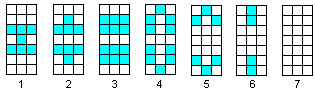
\includegraphics[width=0.6\textwidth]{./inf/SEKII/18_Java_Arrays/GoL1.png}
\end{center}

Weitere Informationen und (teilweise animierte) Beispiele findest in der Datei
\myFile{Game\_of\_Life.html} im Kurs-Repository. Du kannst die Datei direkt in
Eclipse öffnen.

\pagebreak

Führe zunächst einige einfache Simulationen per Hand durch:

\begin{tabular}{cccccc}
a) &
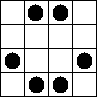
\includegraphics[width=0.15\textwidth]{./inf/SEKII/18_Java_Arrays/GoL2.png} &
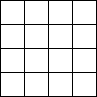
\includegraphics[width=0.15\textwidth]{./inf/SEKII/18_Java_Arrays/GoL.png} &
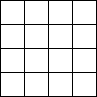
\includegraphics[width=0.15\textwidth]{./inf/SEKII/18_Java_Arrays/GoL.png} &
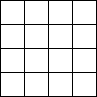
\includegraphics[width=0.15\textwidth]{./inf/SEKII/18_Java_Arrays/GoL.png} &
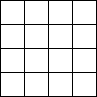
\includegraphics[width=0.15\textwidth]{./inf/SEKII/18_Java_Arrays/GoL.png} \\
b) &
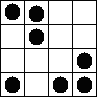
\includegraphics[width=0.15\textwidth]{./inf/SEKII/18_Java_Arrays/GoL3.png} &
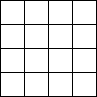
\includegraphics[width=0.15\textwidth]{./inf/SEKII/18_Java_Arrays/GoL.png} &
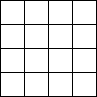
\includegraphics[width=0.15\textwidth]{./inf/SEKII/18_Java_Arrays/GoL.png} &
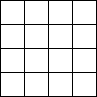
\includegraphics[width=0.15\textwidth]{./inf/SEKII/18_Java_Arrays/GoL.png} &
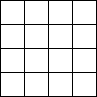
\includegraphics[width=0.15\textwidth]{./inf/SEKII/18_Java_Arrays/GoL.png} \\
c) &
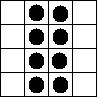
\includegraphics[width=0.15\textwidth]{./inf/SEKII/18_Java_Arrays/GoL4.png} &
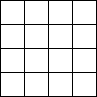
\includegraphics[width=0.15\textwidth]{./inf/SEKII/18_Java_Arrays/GoL.png} &
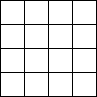
\includegraphics[width=0.15\textwidth]{./inf/SEKII/18_Java_Arrays/GoL.png} &
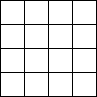
\includegraphics[width=0.15\textwidth]{./inf/SEKII/18_Java_Arrays/GoL.png} &
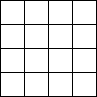
\includegraphics[width=0.15\textwidth]{./inf/SEKII/18_Java_Arrays/GoL.png} \\
d) &
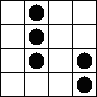
\includegraphics[width=0.15\textwidth]{./inf/SEKII/18_Java_Arrays/GoL5.png} &
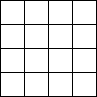
\includegraphics[width=0.15\textwidth]{./inf/SEKII/18_Java_Arrays/GoL.png} &
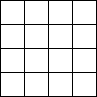
\includegraphics[width=0.15\textwidth]{./inf/SEKII/18_Java_Arrays/GoL.png} &
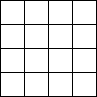
\includegraphics[width=0.15\textwidth]{./inf/SEKII/18_Java_Arrays/GoL.png} &
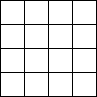
\includegraphics[width=0.15\textwidth]{./inf/SEKII/18_Java_Arrays/GoL.png} \\
e) &
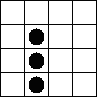
\includegraphics[width=0.15\textwidth]{./inf/SEKII/18_Java_Arrays/GoL6.png} &
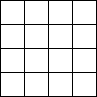
\includegraphics[width=0.15\textwidth]{./inf/SEKII/18_Java_Arrays/GoL.png} &
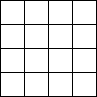
\includegraphics[width=0.15\textwidth]{./inf/SEKII/18_Java_Arrays/GoL.png} &
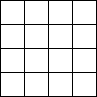
\includegraphics[width=0.15\textwidth]{./inf/SEKII/18_Java_Arrays/GoL.png} &
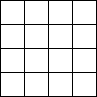
\includegraphics[width=0.15\textwidth]{./inf/SEKII/18_Java_Arrays/GoL.png} \\
\end{tabular}

\subsubsection{Programmieraufgabe}

Schreibe eine Java-Anwendung, die \emph{das Game of Life} simuliert. Gehe in
folgenden Teilschritten vor:

\begin{compactenum}[a)]
\item Zum Testen ist es hilfreich, wenn man anfangs mit wenigen Zellen
arbeitet (z.B. 3*3 Zellen). Wenn alles funktioniert, kann man dann ein großes
Feld erzeugen (z.B. 150*100 Zellen). Definiere deshalb Konstanten, die die
Anzahl der Zellen in x- und in y-Richtung festlegen.  Lege in einer weiteren
Konstanten die Breite einer Zelle fest.

\item Erzeuge ein zweidimensionales boolesches Array, das für jede Zelle
abspeichert ob sie lebendig (\lstinline|true|) oder tot (\lstinline|false|) ist.
Fülle das Array mit zufälligen Anfangswerten.

\item Zeichne die Zellen. Eine lebendige Zelle wird als ausgefülltes Quadrat
gezeichnet. Eine tote Zelle wird als hohles Quadrat gezeichnet.

\item Programmiere eine Methode, die die Anzahl der lebenden Nachbarn einer
Zelle zählt. Dabei wird zunächst davon ausgegangen, dass sich die Zelle in der
Mitte des Feldes befindet (das heißt sie besitzt alle acht Nachbarn). Die
Methode erhält die Koordinaten der Zelle (x- und y-Position) als Parameter
übergeben und gibt die Anzahl der Nachbarn zurück. Teste die korrekte
Funktionsweise der Methode gründlich aus, ehe du weiter arbeitest. Rufe dazu
die Methode für irgendeine Zelle auf (z.B. Zelle (2|1) und überprüfe den
Rückgabewert in dem du die Anzahl der Nachbarn von Hand abzählst.

\item Erweitere die Methode aus Aufgabe (d) so, dass sie auch für Zellen
funktioniert, die sich am Rand des Gitternetzes befinden. Dazu musst du durch
\lstinline|if|-Abfragen sicherstellen, dass beim Zählen der lebenden Nachbarn
niemals Koordinaten von Zellen aufgerufen werden, die nicht existieren. Teste
die Methode für verschiedene Rand-Zellen aus (linker Rand, rechter Rand, oberer
Rand und unterer Rand).

\item Programmiere eine Methode, die entsprechend der Regeln von Conway
berechnet, ob eine bestimmte Zelle im nächsten Zyklus lebt oder nicht. Die
Methode erhält als Parameter die x- und y-Koordinate der Zelle übergeben sowie
die Anzahl ihrer Nachbarzellen (die mit der Methode aus Aufgabe e) ermittelt
wird). Der Rückgabewert ist ein boolescher Wert, der angibt, ob die Zelle im
nächsten Zyklus lebt (\lstinline|true|) oder nicht (\lstinline|false|).

\item Rufe in der myPaint()-Methode des Anwendungsfensters die Methoden aus
Aufgabe e) und f) für jede Zelle des Feldes einmal auf (durch zwei ineinander
geschachtelte Schleifen), um den nächsten Lebenszyklus zu berechnen. Wichtig
ist, dass die neuen „Lebenswerte“ nicht sofort in das boolesche Array
hineingeschrieben werden, weil dann die Berechnung der Nachbarzellen nicht mehr
korrekt erfolgen würde. Deshalb muss ein zweites Array von booleschen Werten
angelegt werden, das die neuen „Lebenswerte“ vorübergehend abspeichert. Nachdem
die neuen „Lebenswerte“ aller Zellen berechnet wurden, werden die booleschen
Werte des Hilfs-Arrays in das echte Array hinüber kopiert. Dazu benötigt man
wieder zwei ineinander geschachtelte Schleifen um jeden Wert einzeln zu
kopieren. Anschließend wird das veränderte Feld mit dem in c) programmierten
Code erneut gezeichnet.

\item Füge in das Anwendungsfenster ein Objekt der Klasse \myClass{Timer} ein,
damit die \lstinline|myPaint()|-Methode in regelmäßigen Zeitabständen aufgerufen
wird, um einen neuen Lebenszyklus zu berechnen.
\end{compactenum}


\subsection{Aufgabe 7: Mandelbrot-Menge}

Ende der achtziger und Anfang der neunziger Jahre des letzten Jahrhunderts
erzeugte nicht zuletzt dank eines Bremer Wissenschaftlers (Heinz-Otto Peitgen,
seit 2013 Präsident der Jacobs University Bremen) die sogenannte \glqq
Chaos-Forschung\grqq\ viel Aufmerksamkeit -- auch in der breiteren
Öffentlichkeit. Nicht zuletzt dürfte das an den faszinierenden Bildern gelegen
haben, die veröffentlicht wurden.

\begin{center}
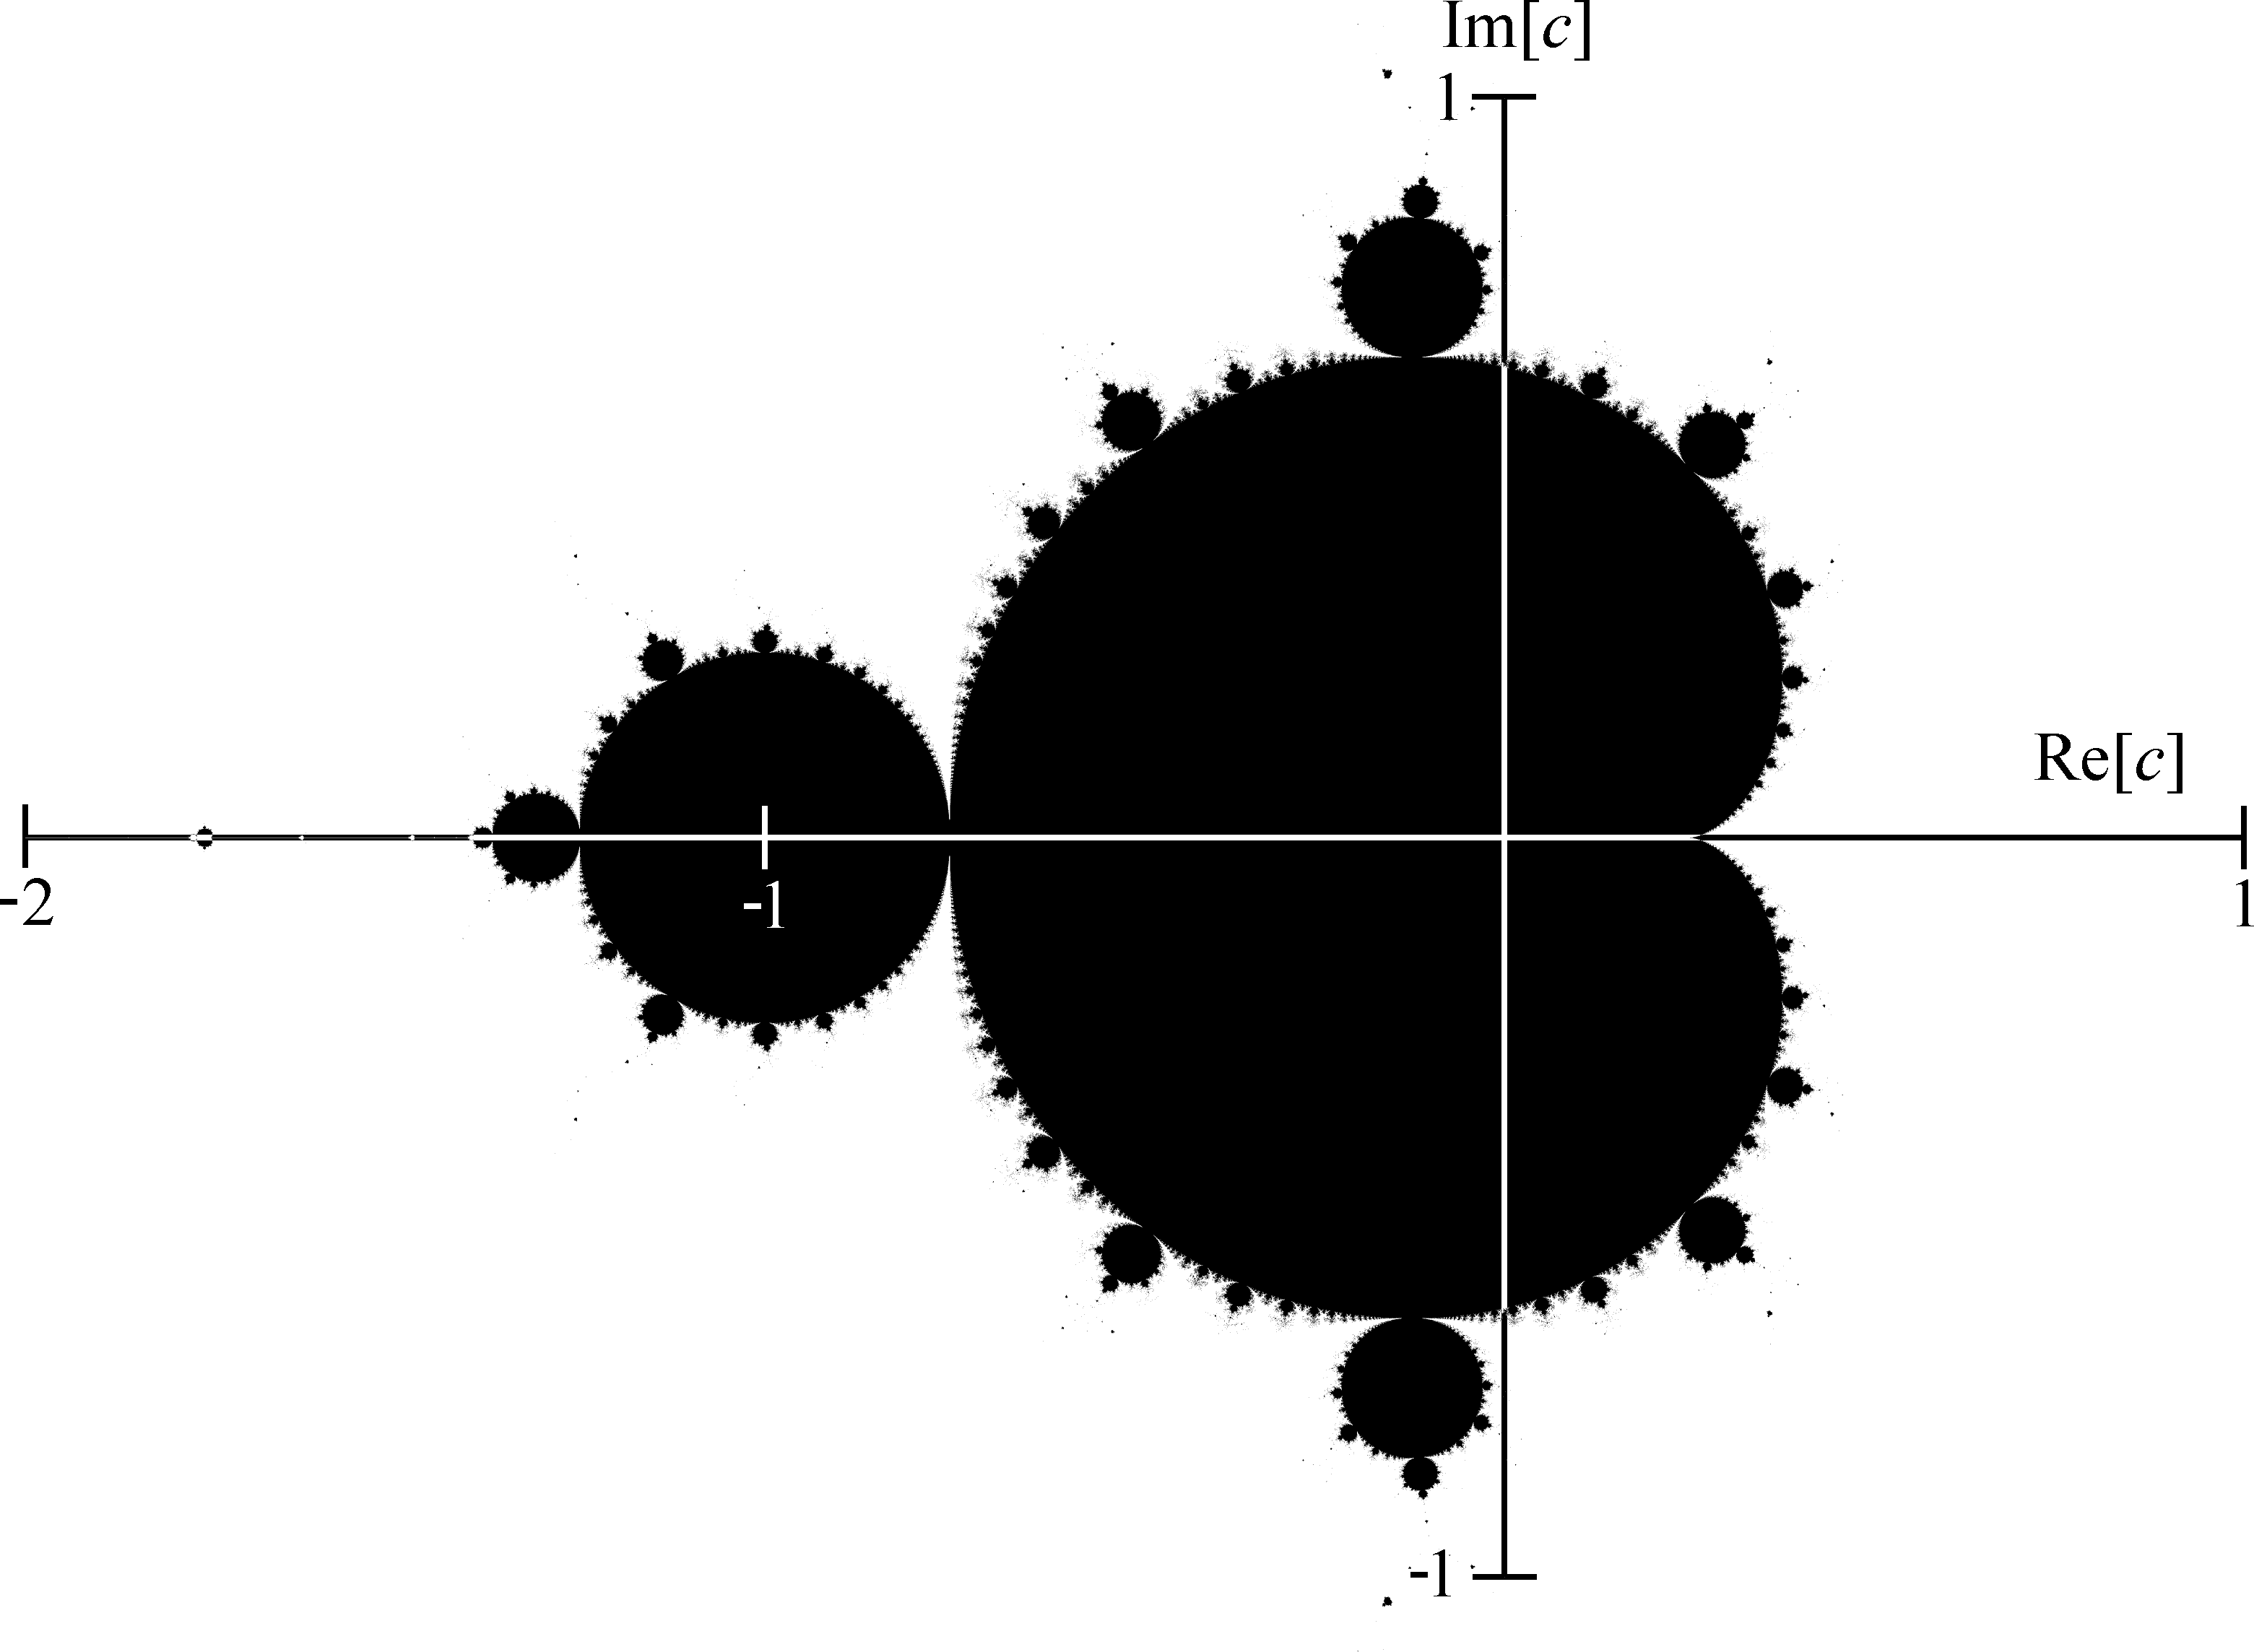
\includegraphics[width=1.0\textwidth]{./inf/SEKII/18_Java_Arrays/Mandelset.png}
% http://commons.wikimedia.org/wiki/File:Mandelset_hires.png
% Public Domain
\end{center}

Das die Chaos-Forschung damals solch einen Aufschwung genommen hat, hängt eng
mit der Entwicklung immer leistungsfähigerer Computer und -- in diesem
Zusammenhang bestimmt ebenso wichtig -- auch geeigneter Ausgabegeräte
(hochauflösende Grafikbildschirme) zusammen. Noch zehn Jahre zuvor hätten die
technischen Möglichkeiten noch nicht gereicht.

Die Mandelbrot-Menge (deren Darstellung oft als \glqq Apfelmännchen\grqq\
bezeichnet wird) war dabei der populärste Betrachtungsgegenstand.

Das auch viele Hobby-Programmierer sich seit damals gerne dem Apfelmännchen
widmen, liegt neben der Schönheit der resultierenden Grafiken sicher auch daran,
dass die Berechnungen ziemlich einfach zu implementieren sind.

Wenn man verstehen will, was bei der Berechnung passiert (was nicht unbedingt
nötig ist), dann muss man zunächst wissen was komplexe Zahlen sind. Die Zahlen,
die ihr aus der Schule kennt sind ganze Zahlen, rationale oder auch irrationale
Zahlen. All diesen Zahlen ist gemein, dass man sie auf einem Zahlenstrahl --
also in einer Dimension -- darstellen kann. Bei den komplexen Zahlen kommt eine
zweite Dimension hinzu. Neben dem uns bereits bekannten reellen Anteil (das was
wir als Zahlen auf dem Zahlenstrahl bereits kennen), kommt ein imaginärer Anteil
hinzu. Die Menge der komplexen Zahlen wird nicht auf einem Zahlenstrahl,
sondern in einer Ebene Dargestellt:

\begin{center}
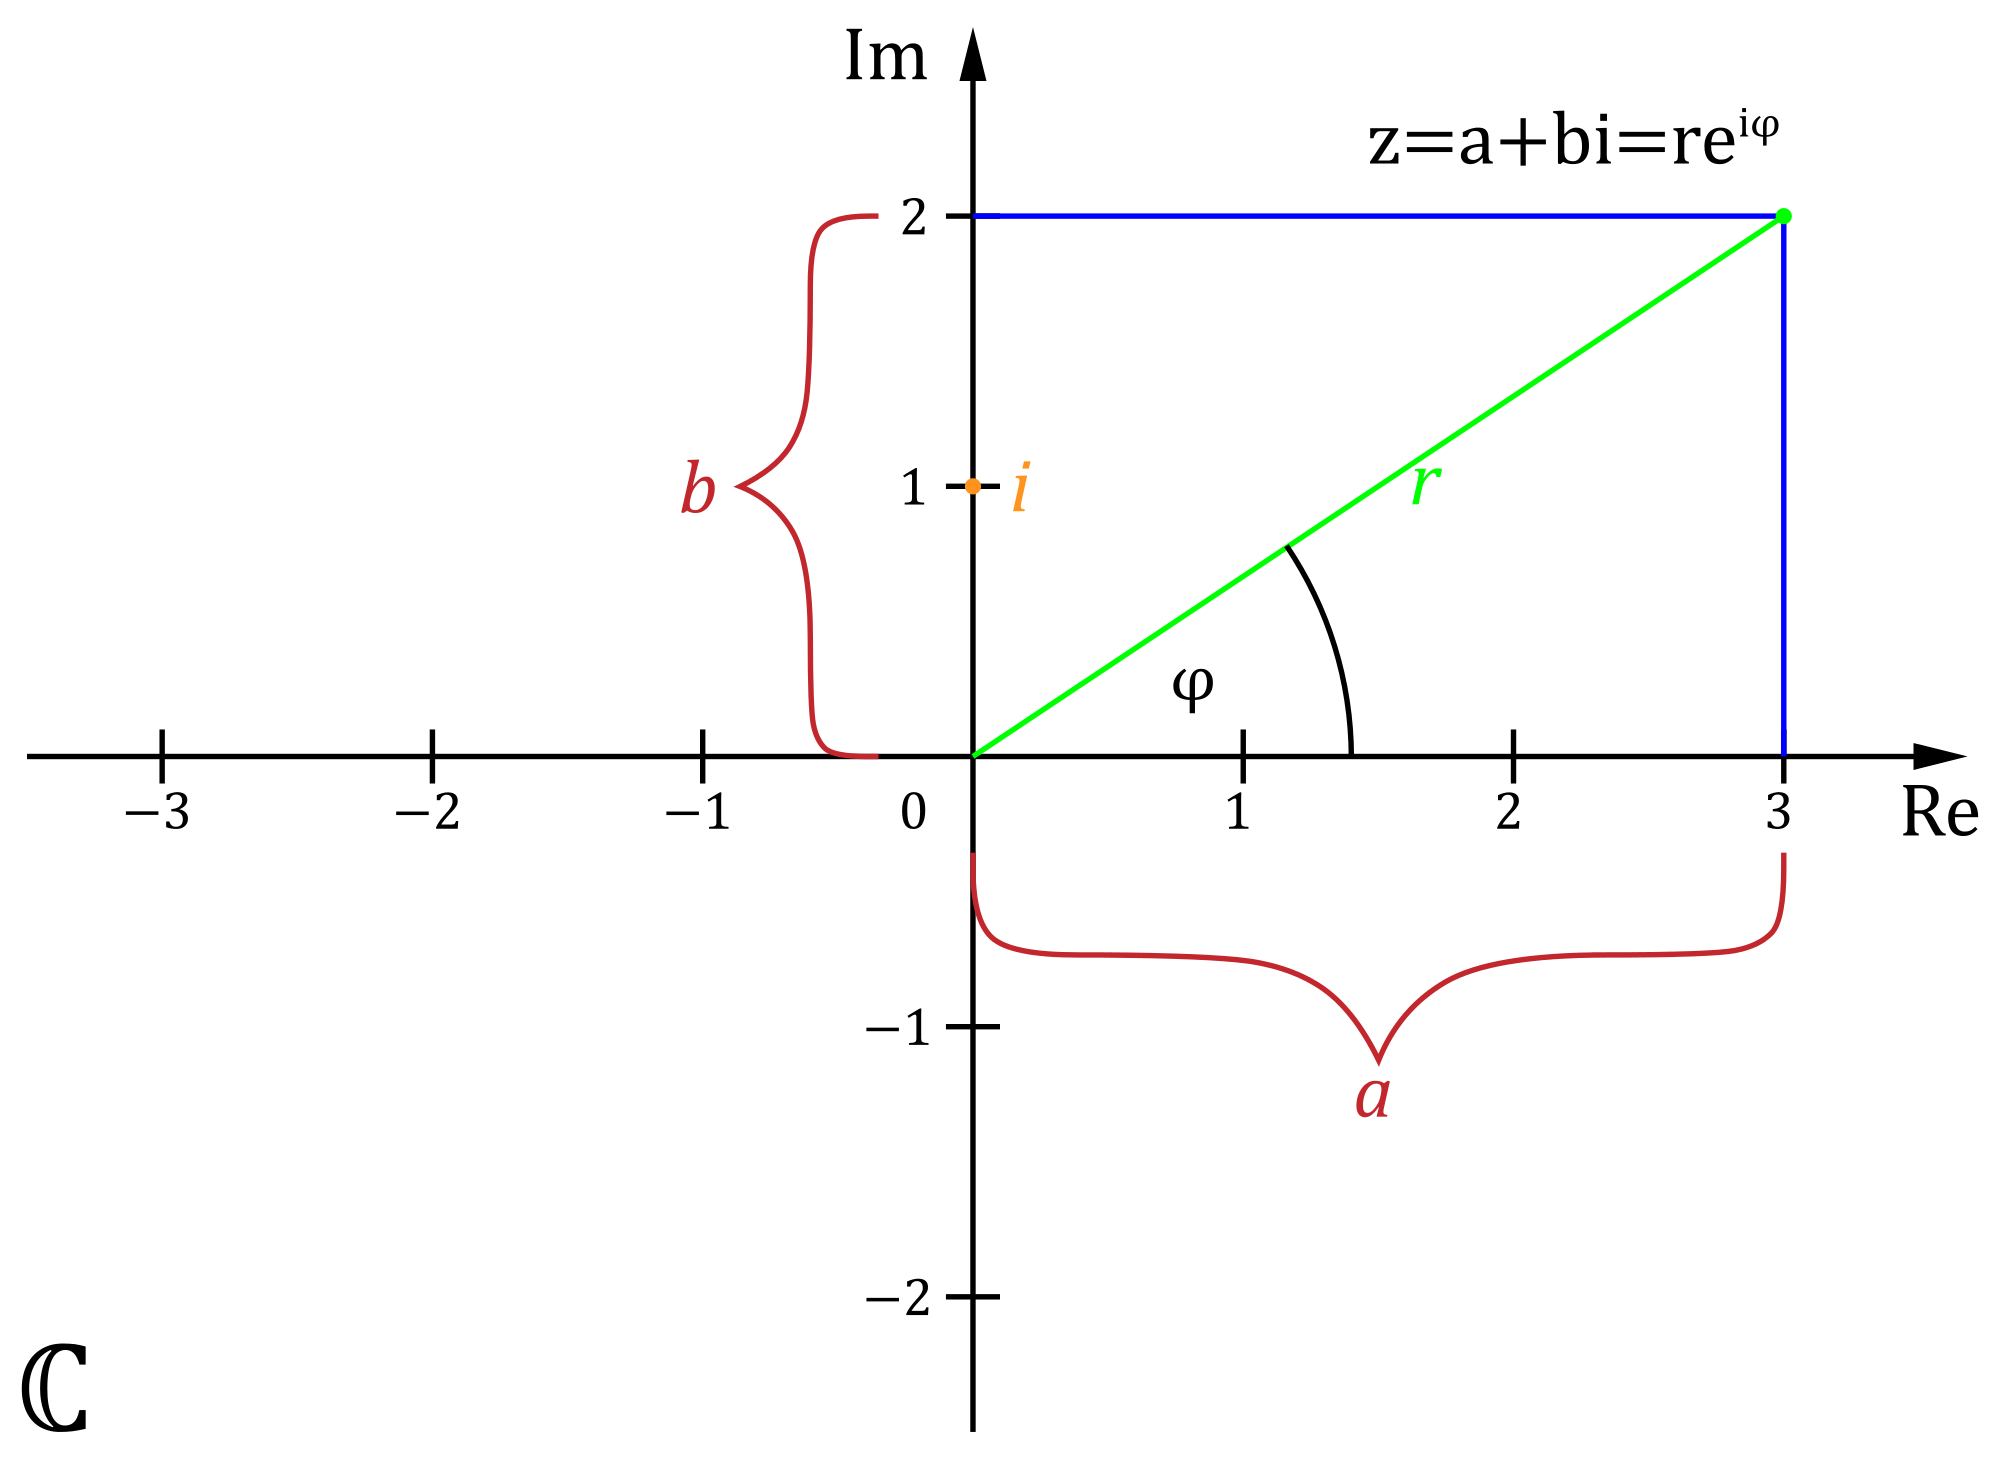
\includegraphics[width=0.45\textwidth]{./inf/SEKII/18_Java_Arrays/Komplexe_Zahlenebene.png}
% http://commons.wikimedia.org/wiki/File:Gaußsche_Zahlenebene.svg
% Public Domain
\end{center}

Die komplexe Zahlen $c$ besteht aus dem Realteil $x$ und dem Imaginärteil $y$.
Man kann schreiben

\[
c = x + i \cdot y
\]

Die Komplexe Zahl ist also die Summe aus ihrem Realteil und dem reellen
Vielfachen der imaginären Einheit $i$. Mit $i = \sqrt{-1}$.


Unsere \glqq normalen\grqq\ Zahlen sind damit ein Sonderfall der
komplexen Zahlen, nämlich die komplexen Zahlen mit dem Imaginärteil 0.

Die Ebene der komplexen Zahlen lässt sich problemlos in einem uns bereits gut
vertrauten Koordinaten-System abbilden: Auf der x-Achse wird dann der Realteil
und auf der y-Achse der Imaginärteil der komplexen Zahl aufgetragen. Da
jedes Pixel auf dem Bildschirm durch eine x- und eine y-Koordinate
beschrieben wird kann man auch jedem Pixel einer komplexen Zahl zuordnen.
Lediglich die Wahl des Ausschnitts aus der komplexen Zahlenebene muss noch
verabredet werden um eine eindeutige Zuordnung von Bildschirmkoordinaten zu
komplexen Zahlen zu bekommen.

Das Apfelmännchen berechnet man, in dem man für jeden Bildpunkt (genauer: für
die komplexe Zahl, die dem Bildpunkt entspricht) die Folge

\begin{equation}
z_{n+1} = z_n^2 + c
\label{eq:mandelbrot}
\end{equation}

und dem Anfangsglied $z_0 = 0$ berechnet. Die Folgeglieder $z_n$ sind
komplexe Zahlen. $c$ ist die komplexe Zahl, die der jeweiligen
Bildschirmkoordinate entspricht.

Für jeden Bildpunkt muss diese Folge berechnet werden und die Frage beantwortet
werden: strebt die Folge ins Unendliche oder bleibt sie beschränkt? Dazu
betrachtet man den Betrag der Folgeglieder.

Der Betrag einer komplexen Zahl ist definiert als

\[
\sqrt{x^2 + y^2}
\]

Soviel zum mathematischen Hintergrund.

In Java rechnen wir nicht mir komplexen Zahlen, sondern mit reellen Zahlen
(\lstinline|double|). Für jede komplexe Zahl brauchen wir zwei reelle Zahlen:
eine für den Realteil und die andere für den Imaginärteil. Oder anders
ausgedrückt: eine für die x-Koordinate und eine für die y-Koordinate.

Der Realteil der Folgeglieder berechnet sich nach

\[
x_{n+1} = x_n^2 + y_n^2 + c_x
\]

und der Imaginärteil nach

\[
y_{n+1} = 2 \cdot x_n \cdot y_n + c_y
\]

Die Frage lautete ja: Ist die Folge für den gewählten Punkt in der komplexen
Zahlenebene beschränkt oder strebt sie ins Unendliche? 

Man hat heraus gefunden, dass \ref{eq:mandelbrot} nach unendlich strebt, wenn
der Betrag der Folgenglieder den Wert 4 übersteigt. Die Berechnung der
Folgeglieder kann also abgebrochen werden, sobald der Betrag größer als 4
geworden ist. Das spart viel Rechenzeit!

Aber was ist, wenn die Folge diesen Grenzwert noch nicht überschritten hat. Es
ist durchaus möglich, dass sie es später noch tun wird! Um diese Frage
einwandfrei zu klären, müsste man im Zweifelsfall unendlich viele Folgeglieder
berechnen. Unendlich viele Folgeglieder sind aber selbst für sehr schneller
Computer zu viel. Also müssen wir die Berechnung auf eine endliche Anzahl von
Folgegliedern beschränken. Dabei gilt es einen Kompromiss zu finden: je mehr
Folgeglieder berechnet werden, desto genauer wird das Ergebnis. Andererseits
steigt der Rechenaufwand.

In Java übersetzt lässt sich die Folge \ref{eq:mandelbrot} so berechnen:

\begin{lstlisting}
public int punktIteration(double cx, double cy, double maxBetragQuadrat, int maxIter) { 
    double betragQuadrat = 0.0;
    int iter = 0;
    double x = 0.0;
    double y = 0.0;
    double xTemp;

    while ((betragQuadrat <= maxBetragQuadrat) && (iter < maxIter)) {
        xTemp = x * x - y * y + cx;
        y = 2 * x * y + cy;
        x = xTemp;
        iter++;
        betragQuadrat = x * x + y * y;
    }

    if (betragQuadrat <= maxBetragQuadrat) {
        iter = 0;
    }
    return iter;
}
\end{lstlisting}

Dabei ist \lstinline|maxBetragQuadrat| der Grenzwert, ab dessen Erreichen wir
davon ausgehen, dass die Folge ins Unendliche strebt. Und \lstinline|maxIter|
ist die Anzahl der Iterationen nach denen die Berechnung abgebrochen werden
soll.

Als Ergebnis liefert die Methode die Anzahl der Iterationen zurück, die sie
durchgeführt hat. Das Ergebnis kann Werte zwischen 0 und \lstinline|maxIter|
annehmen. Je größer der Rückgabewert ist, desto länger hat die Folge gebraucht
um ins Unendliche zu entweichen. Der Rückgabewert 0 ist ein Sonderfall: Wenn du
dir die Methode \lstinline|punktIteration()| anschaust, dann siehst du, dass
dieser Wert genau dann zurück gegeben wird, wenn die Folge es auch nach
\lstinline|maxIter| Iterationen noch nicht geschafft hat den Grenzwert
\lstinline|maxBetragQuadrat| zu erreichen -- wir also davon ausgehen, dass die
Folge für diesen Startwert beschränkt bleibt (nicht ins Unendliche strebt).


\subsubsection{Programmieraufgabe}

Erzeuge ein zweidimensionales Array von \lstinline|int|-Werten von 800 mal 600.
Dieses entspricht dann einer Zeichenfläche von 800 mal 600 Pixeln.

Die Zeichenfläche soll dem Bereich der komplexen Zahlen von -2.2 bis 1.1
(Realteil) und -1.25 bis 1.25 (Imaginärteil) entsprechen. Du musst also später
für die Berechnung Pixelkoordinaten in Real- und Imaginärteil der komplexen Zahl
$c$ \glqq übersetzen\grqq .

Nun muss für jedes Element des zweidimensionalen Arrays die Methode
\lstinline|punktIteration()| aufgerufen werden und der Rückgabewert in dem
Arrayelemnt gespeichert werden.

In der \lstinline|myPaint()|-Methode liest du die Array-Elemente aus und weist
dem zugehörigen Bildpunkt auf der Zeichenfläche einen Farbwert in Abhängigkeit
vom Wert des Array-Elements zu. Im einfachsten Fall lässt du für alle
Array-Elemente, die den Wert 0 enthalten einen schwarzen Punkt
an der entsprechenden Koordinate auf der Zeichenfläche zeichnen (etwa mit der
\myClass{Graphics}-Methode \lstinline|fillRect()|, wobei du als Breite und Höhe
jeweils genau ein Pixel angibst), und alle anderen Bildpunkte lässt du weiß.

Wenn du es hübscher willst, dann dann weist du den Punkten, die größere Werte
als 0 haben (die also ins Unendliche divergiert sind), einen Farbwert zu, der
abhängig vom tatsächlichen Wert ist. Etwa Grauwerte, die umso dunkler sind, je
länger der Punkt gebraucht hat um ins Unendliche zu entkommen. Natürlich geht
das auch farbig.

Wenn es dir so gelungen ist ein Apfelmännchen auf den Bildschirm zu zeichnen
kannst du anfangen zu experimentieren (andere Bildausschnitte, andere
Rechentiefen, andere Farbgebung).

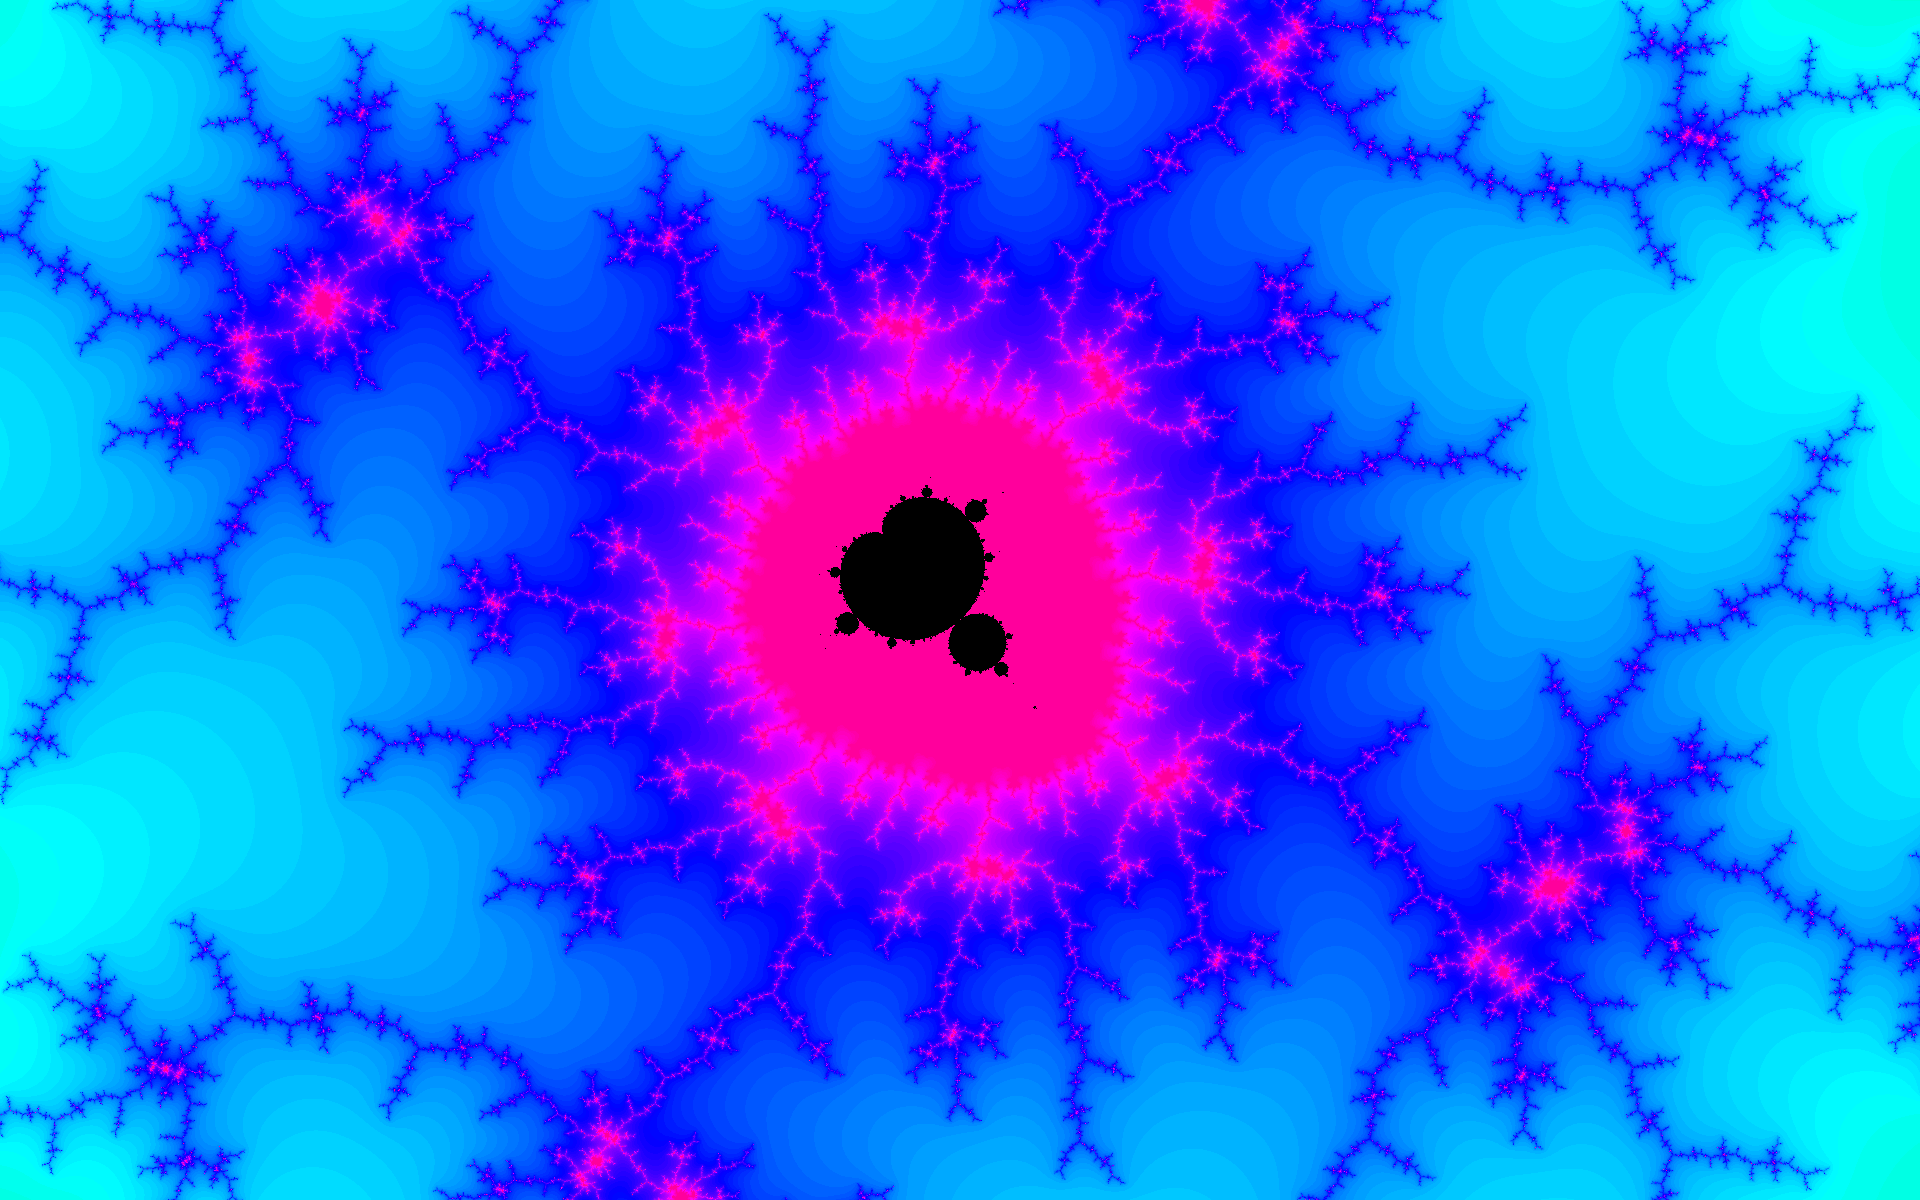
\includegraphics[width=1.0\textwidth]{./inf/SEKII/18_Java_Arrays/mandelbrot_1.png}
% http://commons.wikimedia.org/wiki/File:Gaußsche_Zahlenebene.svg
% Public Domain

Hinweis: \lstinline|maxIter| sollte mindestens den Wert 100 haben. Je tiefer du
in die Mandelbrot-Menge hinein zoomst (je kleiner der Ausschnitt ist, den du
betrachtest), desto höheren Rechenaufwand musst du betreiben um die dann
sichtbar werdenden feinen Details noch auflösen zu können. Der Wert für
\lstinline|maxIter| muss also größer werden, je stärker du \glqq
vergrößern\grqq\ möchtest.


\subsection{Aufgabe 8: Clifford-Attraktor}

Betrachte die Gleichungen

\begin{eqnarray}
x_{n+1} &=& \sin (a \cdot y_n) + c \cdot \cos (a \cdot x_n)
\label{eq:clifford1}\\
y_{n+1} &=& \sin (b \cdot x_n) + d \cdot \cos (b \cdot x_n)
\label{eq:clifford2}
\end{eqnarray}

Du siehst hier zwei Folgen, die zum einen voneinander abhängig sind ($y_{n+1}$
ist abhängig von $x_n$ und $x_{n+1}$ ist abhängig von $y_n$). Außerdem gibt es
noch vier Parameter: $a$, $b$, $c$ und $d$.

Wenn man den Verlauf der Folgenglieder betrachtet, so stellt man fest, dass
diese sich (bei gegebenen Parametern $a$, $b$, $c$ und $d$) -- unabhängig vom
gewählten Startpunkt -- auf festen, wenn auch teilweise recht chaotischen Bahnen
bewegen. Wobei der Begriff \glqq Bahn\grqq\ etwas irreführend ist, da er
suggeriert die Folgeglieder würden Schritt für Schritt diese Bahn abschreiten.
Dem ist jedoch keineswegs so: Vielmehr springen die Folgeglieder \glqq
wild\grqq\ umher, landen bei diesen Sprüngen aber immer wieder auf dieser \glqq
Bahn\grqq .

Solch ein \glqq anziehendes\grqq\ Verhalten wird als \emph{Attraktor}
bezeichnet.

\begin{center}
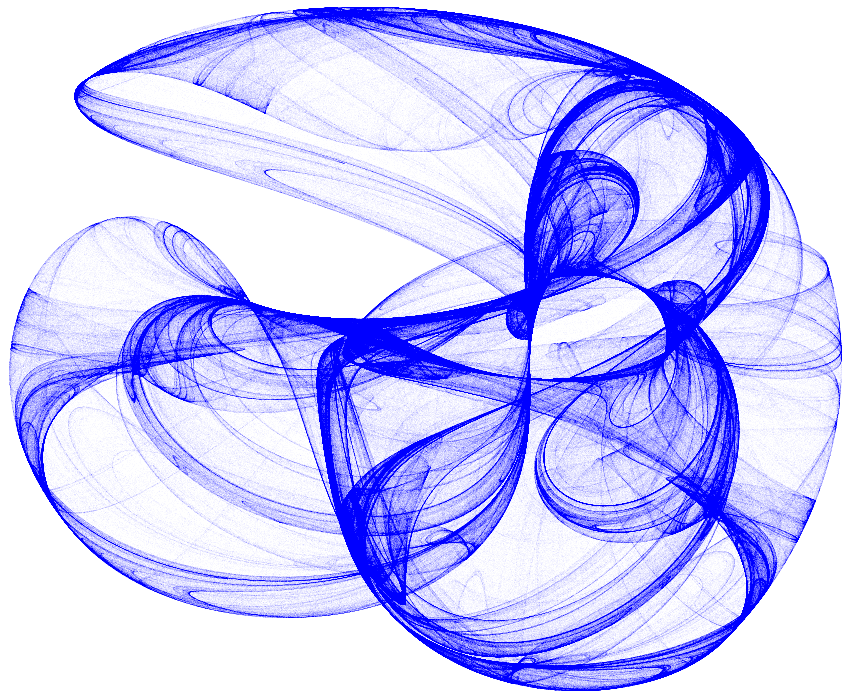
\includegraphics[width=1.0\textwidth]{./inf/SEKII/18_Java_Arrays/clifford.png}
% selbst erstellt
\end{center}

Die Abbildung zeigt einen nach Ihrem \glqq Entdecker\grqq\ Clifford
Pickover benannten Clifford-Attraktor (manchmal auch Pickover-Attraktor
genannt) der auf den Gleichungen \ref{eq:clifford1} und \ref{eq:clifford2}
basiert. Als Parameter wurden dabei gewählt: $a=1.1$, $b=-1.0$, $c=1.8$ und
$d=1.5$


\subsubsection{Programmieraufgabe}

Gehe vor wie für das Apfelmännchen beschrieben: Berechne eine große (aber
endliche) Anzahl von Folgegliedern.

Für einen ersten Eindruck reichen eine halbe Million Iterationen. Für ein
schönes Ergebnis sollten es schon zehn Millionen Iterationen sein.

Zähle dabei mit, wie oft Folgenglieder auf den einzelnen x- und y- Koordinaten
landen, in dem du in einem zweidimensionalen Array vom Typ \lstinline|int| die
Trefferanzahl hochzählst. Jedes Element dieses Treffer-Arrays gibt anschließend
also Auskunft darüber, wie oft es von der Folge (den x- und
y-Koordinaten, die sich durch die Folgeglieder von  \ref{eq:clifford1} und
\ref{eq:clifford2} definieren) getroffen wurde.

In der \lstinline|myPaint()|-Methode übersetzt du dann die Werte im
Treffer-Array in Farbwerte für die entsprechenden Bildschirmkoordinaten.

Interessant ist die Wahl der Startwerte für die Folgen $x$ und $y$: Du kannst
entweder darauf vertrauen, dass das oben gesagte stimmt, und die Folgeglieder
tatsächlich unabhängig vom Startwert auf dem Attraktor landen, oder du
überprüfst dies, in dem du beispielsweise alle zehntausend Iterationen neue
Startwerte für $x$ und $y$ per Zufallsgenerator erzeugen lässt. Beide Verfahren
sollten zum gleichen Ergebnis führen!

